Data goes through a particular path through the pipeline of a processor and typically, a pipeline is split up in multiple stages. With a lockstep processor, each of the stages are effectively working in parallel. Figure \ref{fig:pipelining} illustrates hardware pipelining for a \emph{Reduced Instruction Set Computer} (RISC) processor. The pipeline is split up in four or more stages, e.g. instruction fetch, instruction decode, execution and write-back stage. During the \emph{instruction fetch} (IF stage) an instruction is loaded from \emph{instruction memory} (IMEM), which is decoded in the \emph{instruction decode} (ID) stage where the type of operation is determined by the opcode and operands are identified by their register addressing, and finally, the operation is executed and the result is written back to the register file.

\begin{figure}[H]
\centering
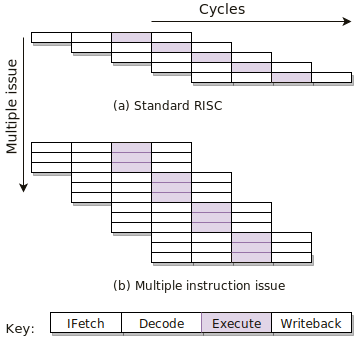
\includegraphics[width=.5\textwidth]{figures/pipelining}
\caption{Pipelining and multiple instruction issue\cite{tta_codegen}.}
\label{fig:pipelining}
\end{figure}

\begin{figure}[b]
\centering
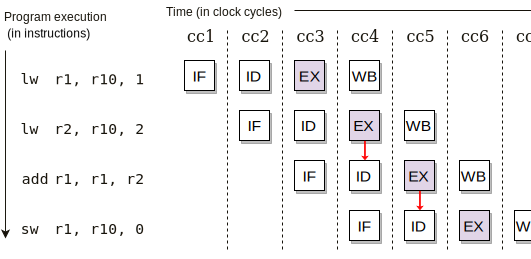
\includegraphics[width=.8\textwidth]{figures/bypassing_example}
\caption{Instructions being executed using the single-cycle datapath, assuming pipelined execution.}
\label{fig:bypass_problem}
\end{figure}

\textbf{Operand forwarding:} When bypassing is completely absent the result of an instruction can only be obtained after it is written back. On the other hand, with bypassing, a bypass network of wires and busses connects the execution and writeback stages back to the ID stage. These wires and busses may be used to forward a value to operands of another instruction. This way, the result of an instruction can be obtained before it has been written back to the register file. This behaviour is illustrated in Figure \ref{fig:bypass_problem}.

Four consecutive instructions are executed of which the last two instructions have a RaW dependency with the instruction prior to it. As you can see in Figure \ref{fig:bypass_problem} the instructions prior to said instructions are in the execution stage when their result is queried, namely, when said instructions are in the ID stage. So either the processor needs to be stalled for a cycle, such that the previous instruction is in the WB stage, or the result needs to be forwarded from the execution stage to the ID stage. Since insertion of stall cycles result in less efficient code, the result is forwarded using the bypass network (indicated with a vertical arrow from EX to ID).

%TODO: update picture, make nicer and have on top stages, and below remain almost the same
%\begin{figure}[H]
%\centering
%\subfloat{\includegraphics[width=.275\textwidth]{figures/bypass_prob_legend}}
%\hfil
%\subfloat{\includegraphics[width=.475\textwidth]{figures/bypass_problem}}
%\caption{Bypassing network differences between four stage and five stage pipeline configuration.}
%\label{fig:bypass_problem}
%\end{figure}
%TODO: replace with picture from presentation (03_nov)
\subsubsection{Implicit Datapaths}
With implicit bypassing (also called transparent bypassing), bypassing opportunities are detected and controlled by dedicated hardware on chip. However, doing this at run-time has some advantages and some disadvantages.
\begin{itemize}
  \item\textbf{Advantage:} 
    With bypassing, operand forwarding is possible which reduces the number of reads from the register file. This will reduce register file usage and may improve energy efficiency of the processor.
  \item\textbf{Disadvantage:} 
    If you push the responsibility of identifying and exploiting forwarding to the hardware, it needs $2\cdot d\cdot n$ comparators (where $d$ is the number of stages between ID en WB and $n$ the number of issue slots) to compare operands of an instruction to registers defined by previous instructions that are already in the pipeline. Altogether, this results in a more complex gate design and increased area.
\end{itemize}

It has been observed that variables in the register file are often transient, meaning that they last only for a short time.  Reads from the register file of said variables can be avoided by forwarding which is shown in the previous paragraphs.\\

Now, we show that register writes of transient values can be avoided with explicit datapaths. The reason why this is only the case for explicit datapaths, and not with implicit bypassing, is that the hardware can only look at instructions that have already been executed, while the compiler can look at all instructions of a program.\\

\textbf{Dead result elimination:} 
If all consumers of a variable obtain it using forwarding, then it will never be read from the register file. Therefore, that variable does not need to be stored in a register file, since it is not read from it anyway. Hence, these obsolete stores may be avoided.  

\subsubsection{Explicit Datapaths}
With explicit datapaths (sometimes referred to as exposed datapaths), bypass opportunities are detected and controlled by the compiler. Doing this at compile time rather than run-time has some advantages and some disadvantages.
\begin{itemize}
  \item\textbf{Advantage:}
    With explicit bypassing, dead result eliminations is possible which reduces the number of writes to the register file. This will further reduce register file usage and may further improve energy efficiency of the processor.
  \item\textbf{Disadvantage:}
    The compiler needs to take datapaths and variables that are in the pipeline into consideration, because bypassing is explicit in the compiler. This results in a more complex compiler.
\end{itemize}

This project focusses on implementing these optimizations for a compiler that targets a wide SIMD architecture. The following section is devoted to explaining the target SIMD architecture.